\section{Closeness}
\FloatBarrier
\begin{figure}[h]
	\centering
	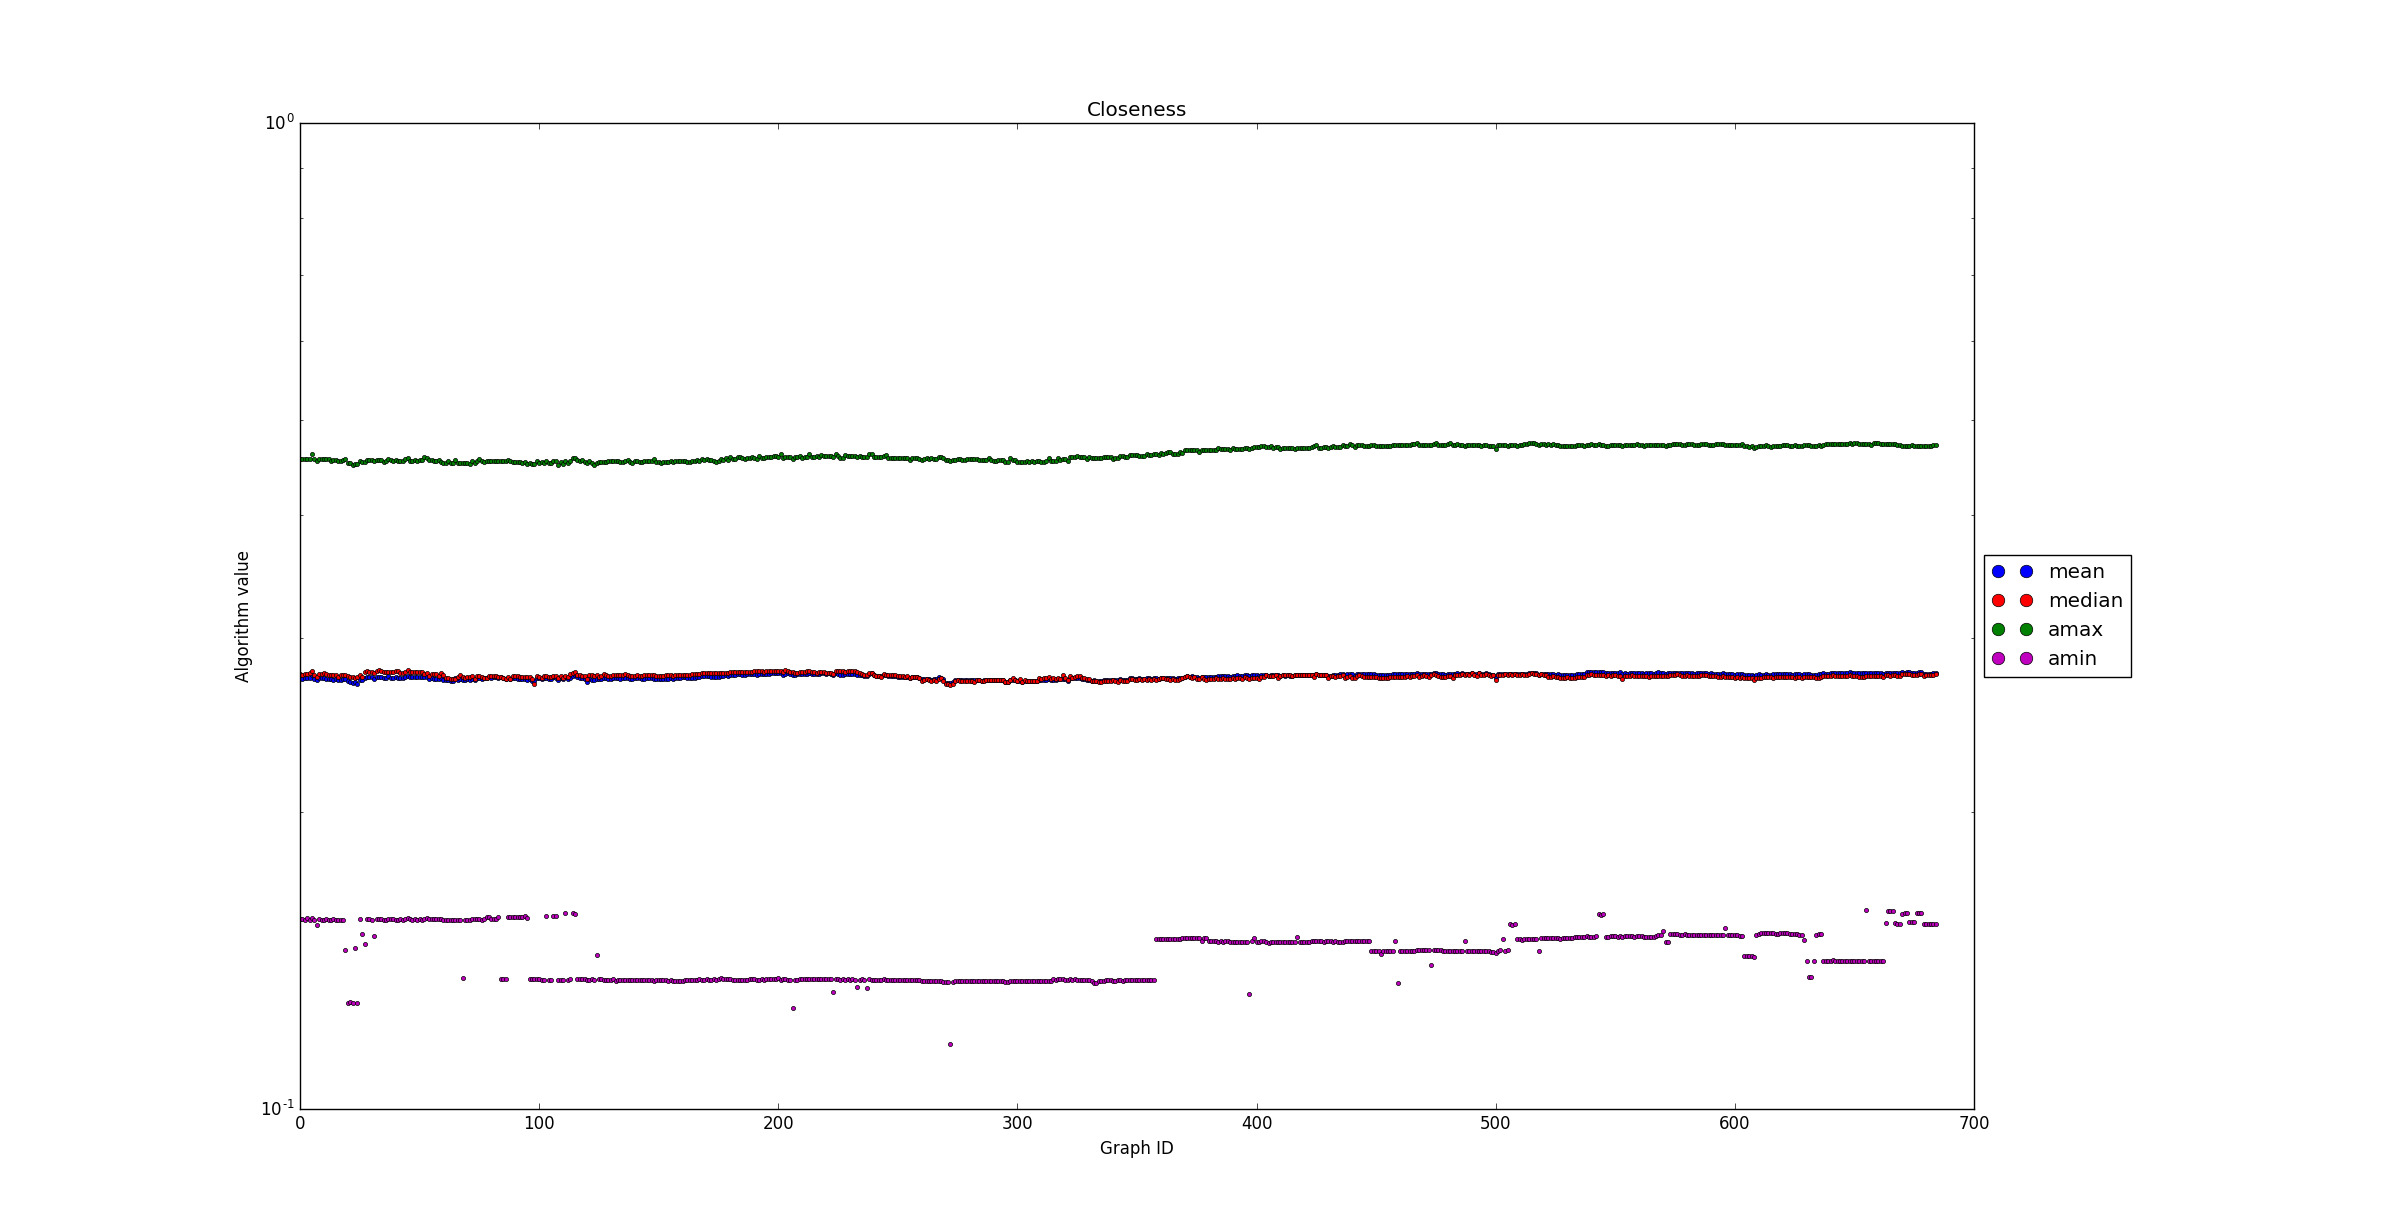
\includegraphics[width=\textwidth]{closeness}
	\caption{Wyniki algorytmu closeness}
\end{figure}
\FloatBarrier\FloatBarrier
\begin{figure}[h]
	\centering
	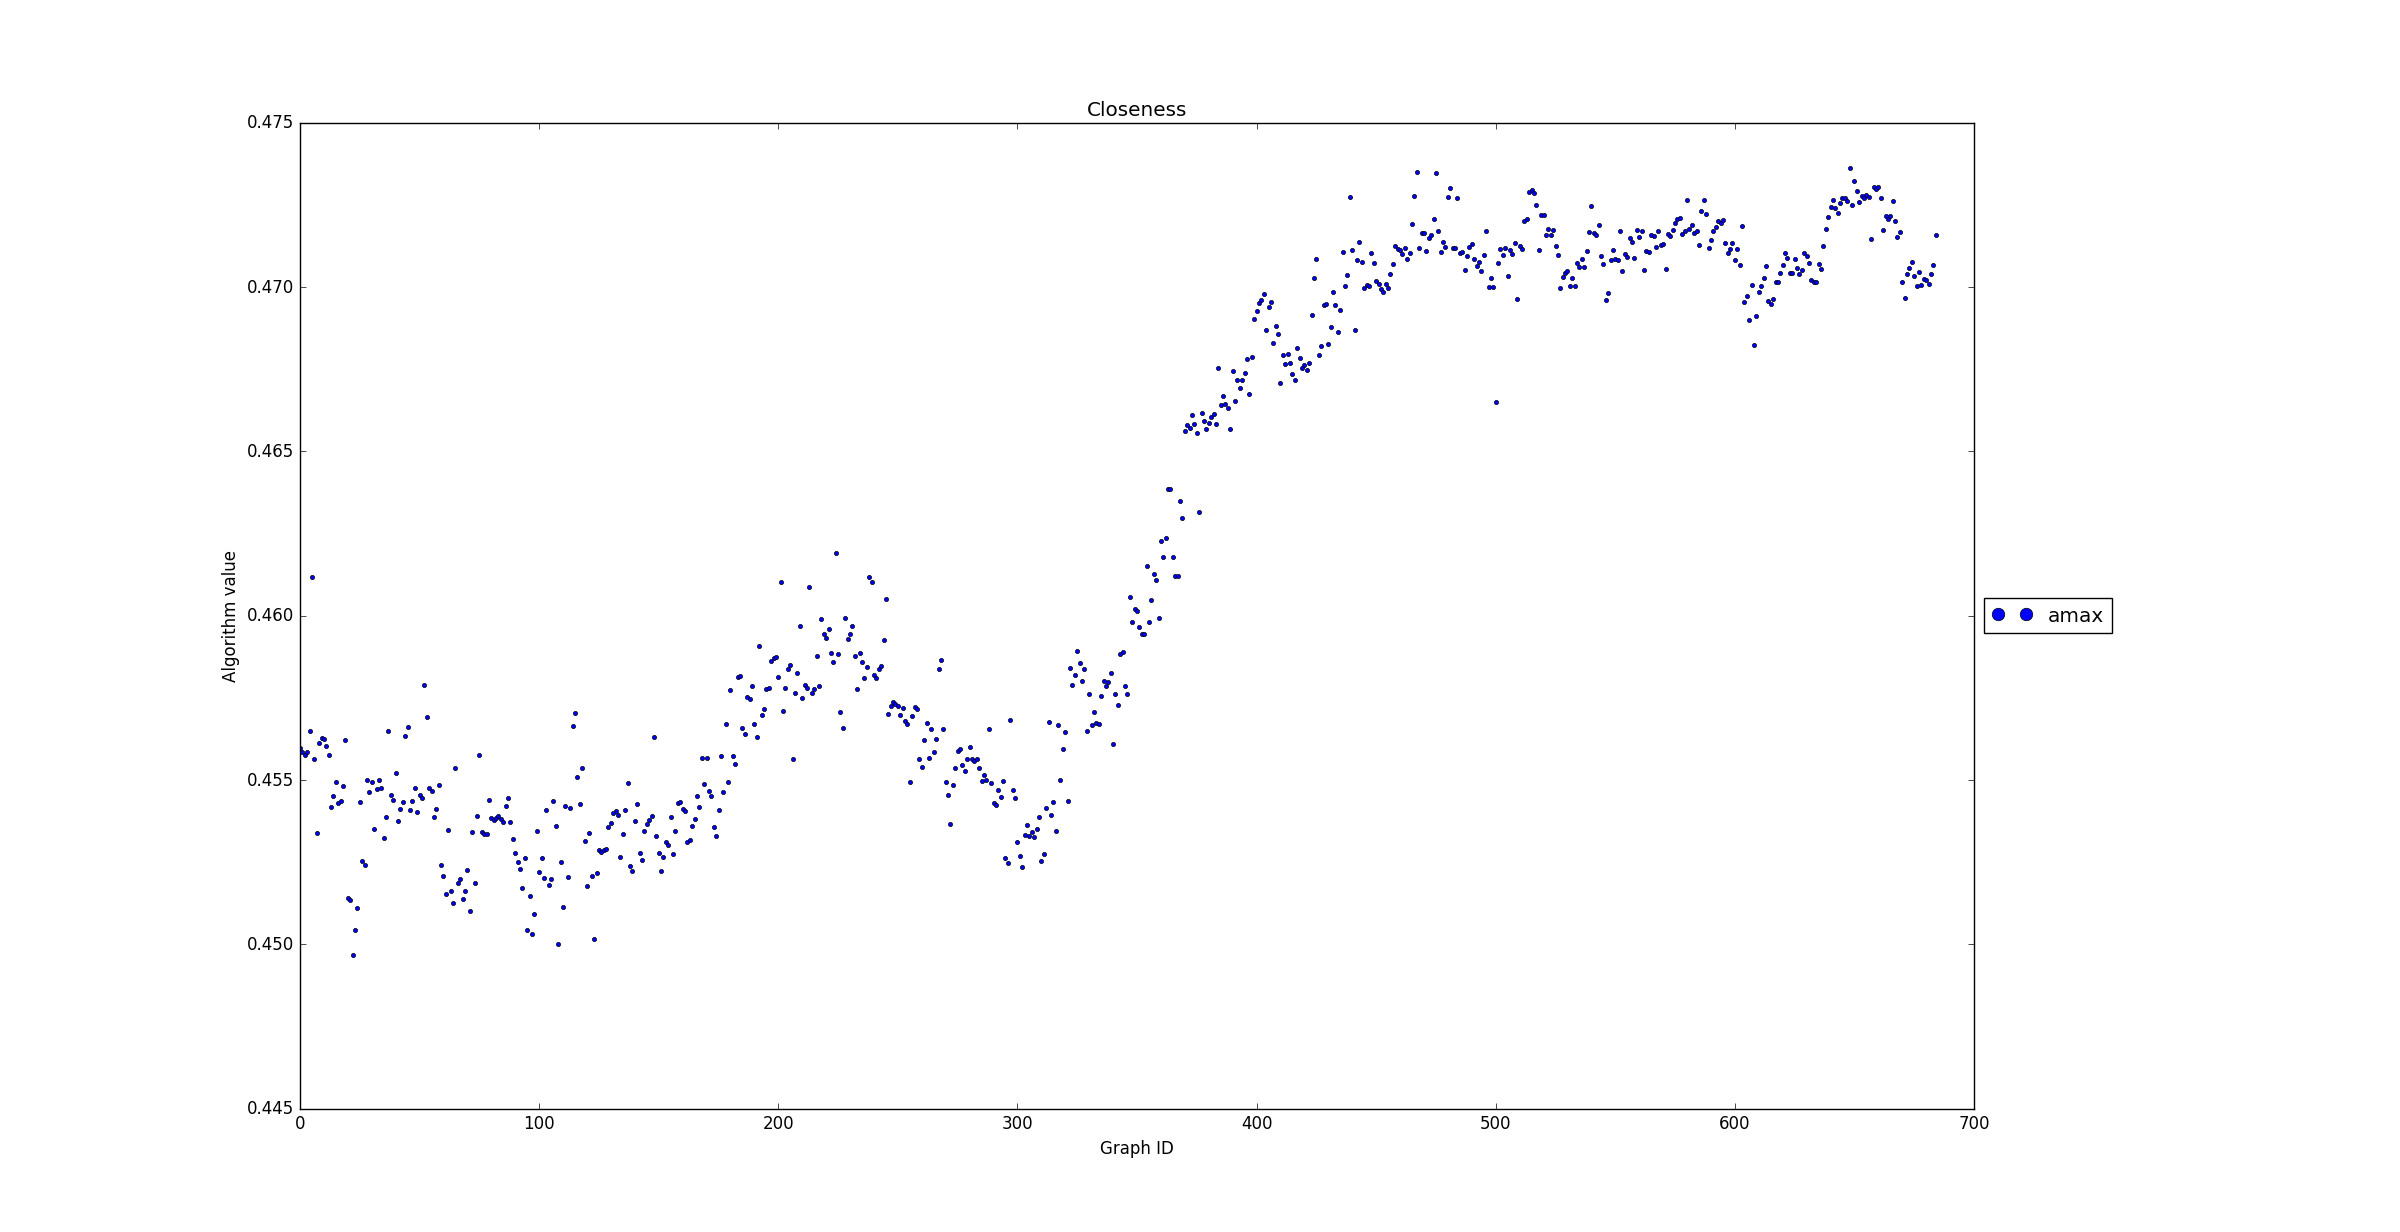
\includegraphics[width=\textwidth]{closeness_max}
	\caption{Maksymalne wartości closeness}
\end{figure}
\FloatBarrier\FloatBarrier
\begin{figure}[h]
	\centering
	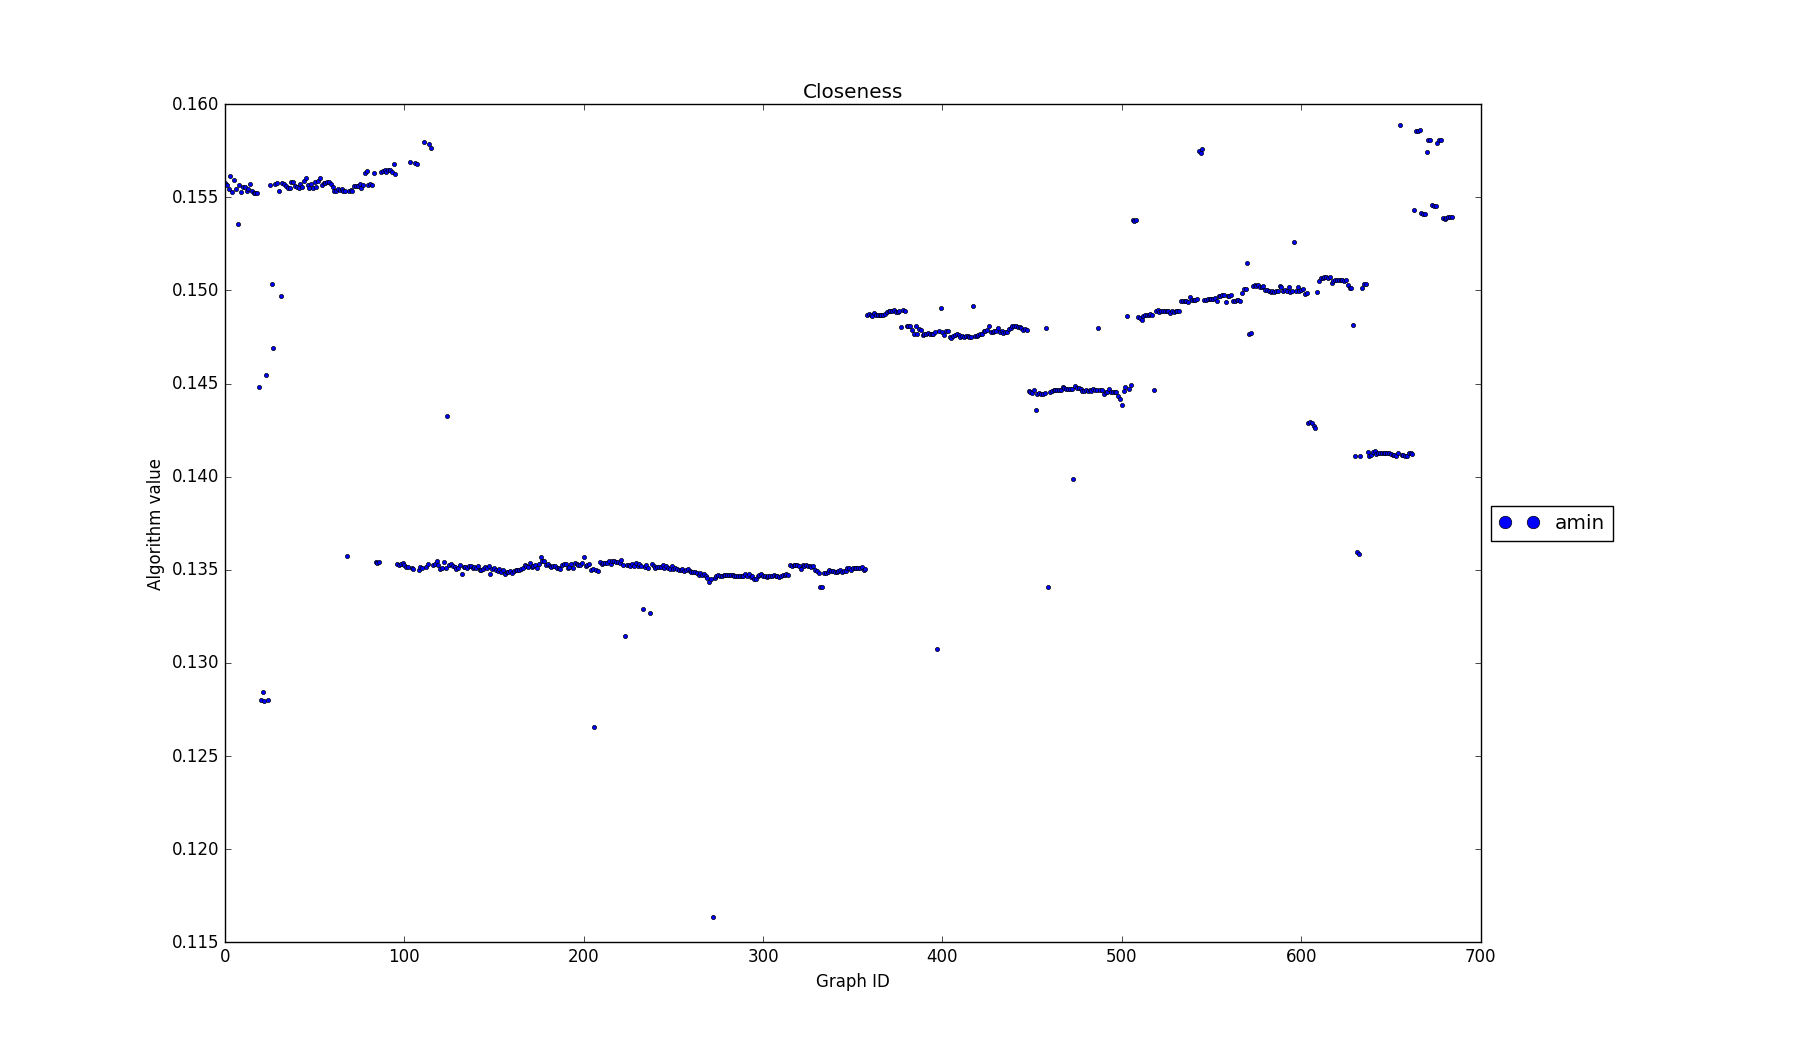
\includegraphics[width=\textwidth]{closeness_min}
	\caption{Minimalne wartości closeness}
\end{figure}
\FloatBarrier\FloatBarrier
\begin{figure}[h]
	\centering
	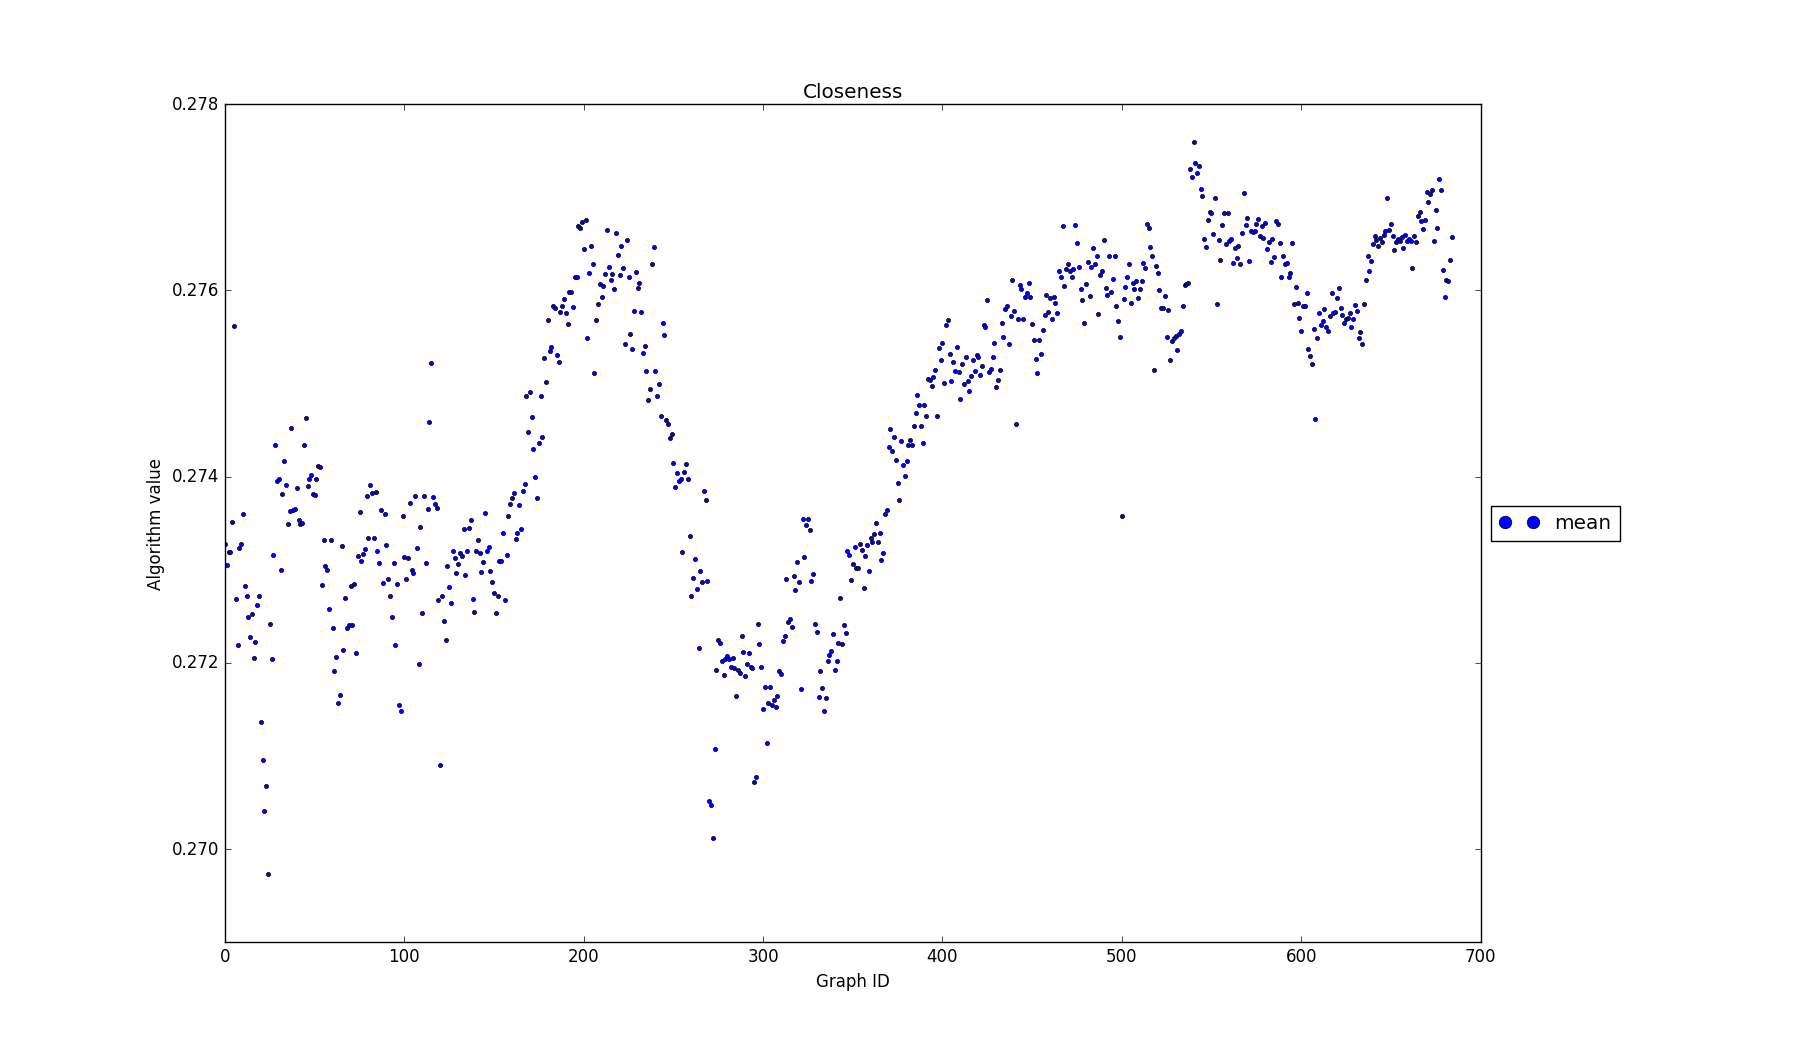
\includegraphics[width=\textwidth]{closeness_mean}
	\caption{Średnie wartości closeness}
\end{figure}
\FloatBarrier\FloatBarrier
\begin{figure}[h]
	\centering
	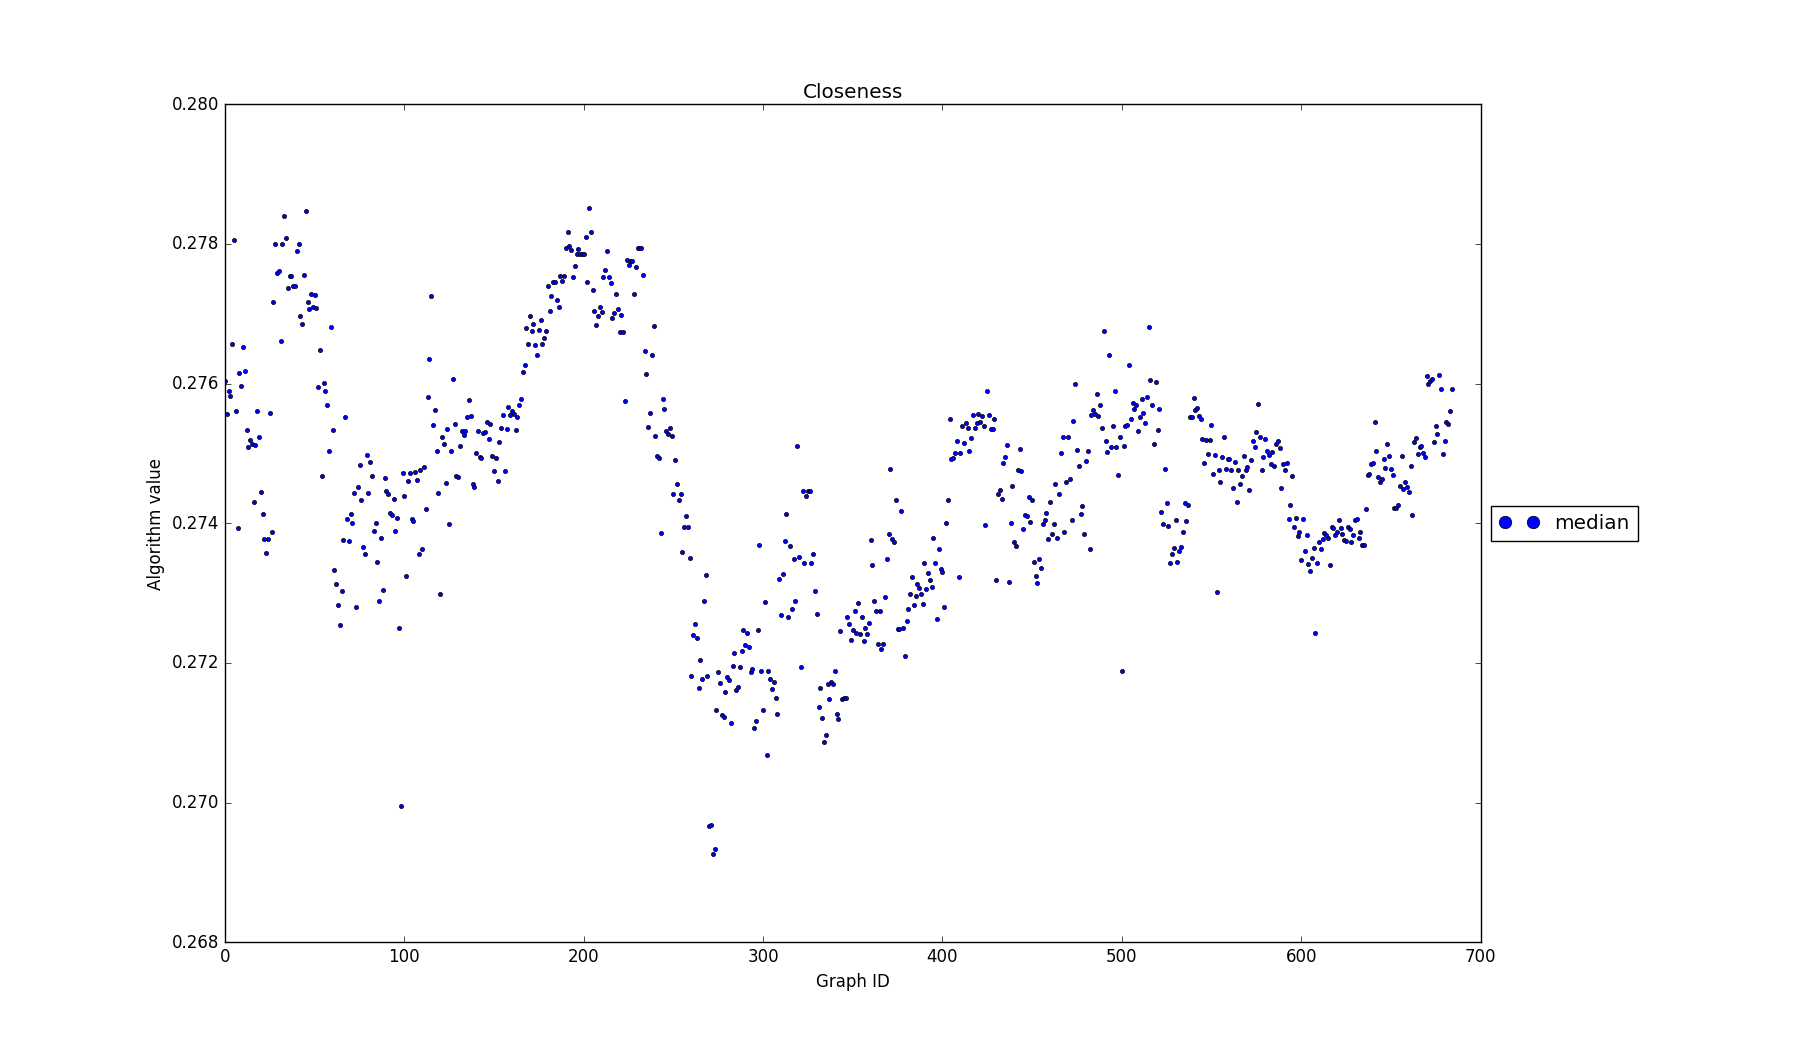
\includegraphics[width=\textwidth]{closeness_median}
	\caption{Mediana wartości closeness}
\end{figure}
\FloatBarrier
Z powyższych wykresów wynika, że na przestrzeni czasu węzły o największych centralnościach powiększyły swoją przewagę nad pozostałymi, tzn. zbliżyły się one do wszystkich węzłów. Świadczyć może o tym przewaga średniej nad medianą w drugiej połowie badanego okresu czasu oraz wyraźny wzrost wartości maksymalnej. Wartość minimalna centralności ma charakterystykę wyraźnie skokową, co świadczyć może o dodaniu innych wierzchołków, najbardziej oddalonych od reszty. 
\newpage
